
\documentclass{bredelebeamer}

%%%%%%%%%%%%%%%%%%%%%%%%%%%%%%%%%%%%%%%%%%%%%%%%

\title[Learning and alcohol dependence]{Learning and alcohol dependence}
\subtitle{From goals to habits: Association with relapse and treatment effectiveness}

\Large\author{\textbf{Alina Koppold}} 
\date{\scriptsize \today}
\institute{
\includegraphics[scale=0.30]{images/Clogo.PNG} \\ \textbf{Emotional neuroscience workgroup}
\\Supervisors: Dr. Miriam Sebold, Prof. Dr. Dr. Andreas Heinz}

\subject{Koppold masterthesis}

%%%%%%%%%%%%%%%%%%%%%%%%%%%%%%%%%%%%%%%%%%%%%%%%%%%%%%%%%%%%%%%%%%%%%

\begin{document}
\begin{frame}
  \titlepage
  
\begin{center}
%
\includegraphics[scale=0.5]{images/Clogo.PNG}\\



\includegraphics[scale=0.15]{images/KUlogo.PNG} \\ 
\scriptsize {Prof. Dr. Marco Steinhauser}

\end{center}
\end{frame}


\begin{frame}{Overwiew}
  \tableofcontents
\end{frame}



%%%%%%%%%%%%%%%%%%%%%%%%%%%%%%%%%%%%%%%%%%%%%%%%%%%%%%%%%%%%%%%%%%%%%%%%%%%%%%%%%%%%%%%%%%%%%%%%%%%%%%%%%%%%%%%%% I N T R O D U C T I O N %%%%%%%%%%%%%%%%%%%%%%%%%%%%%%%%%%
%%%%%%%%%%%%%%%%%%%%%%%%%%%%%%%%%%%%%%%%%%%%%%%%%%%%%%%%%%%%%%%%%%%%%%%%%%%%%%%%%%%%%%
\section{Introduction} 
\subsection{DIE MACHT DER GEWOHNHEIT}

\begin{frame}{Balance of two systems}

    \begin{figure}
        \centering
        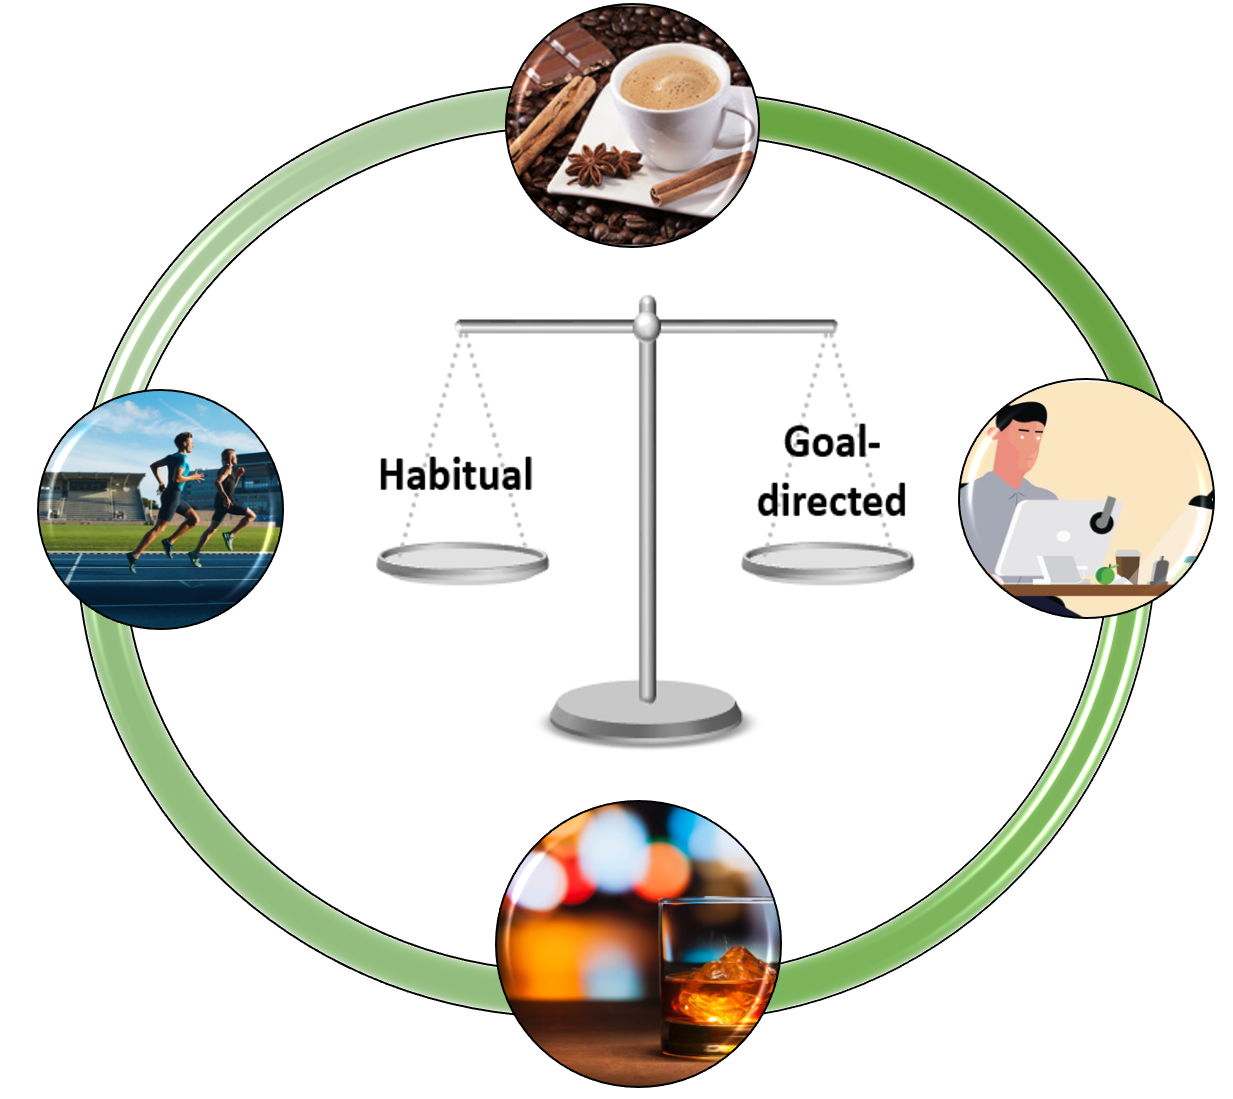
\includegraphics[scale=0.32]{images/gZy.PNG}
        \caption{\small{Dual control approach.}}
    \end{figure}
\end{frame}
%%%%%
\begin{frame}{What do we already know about alcohol dependence and these systems?}
    \centering
     \begin{figure}
        \centering
        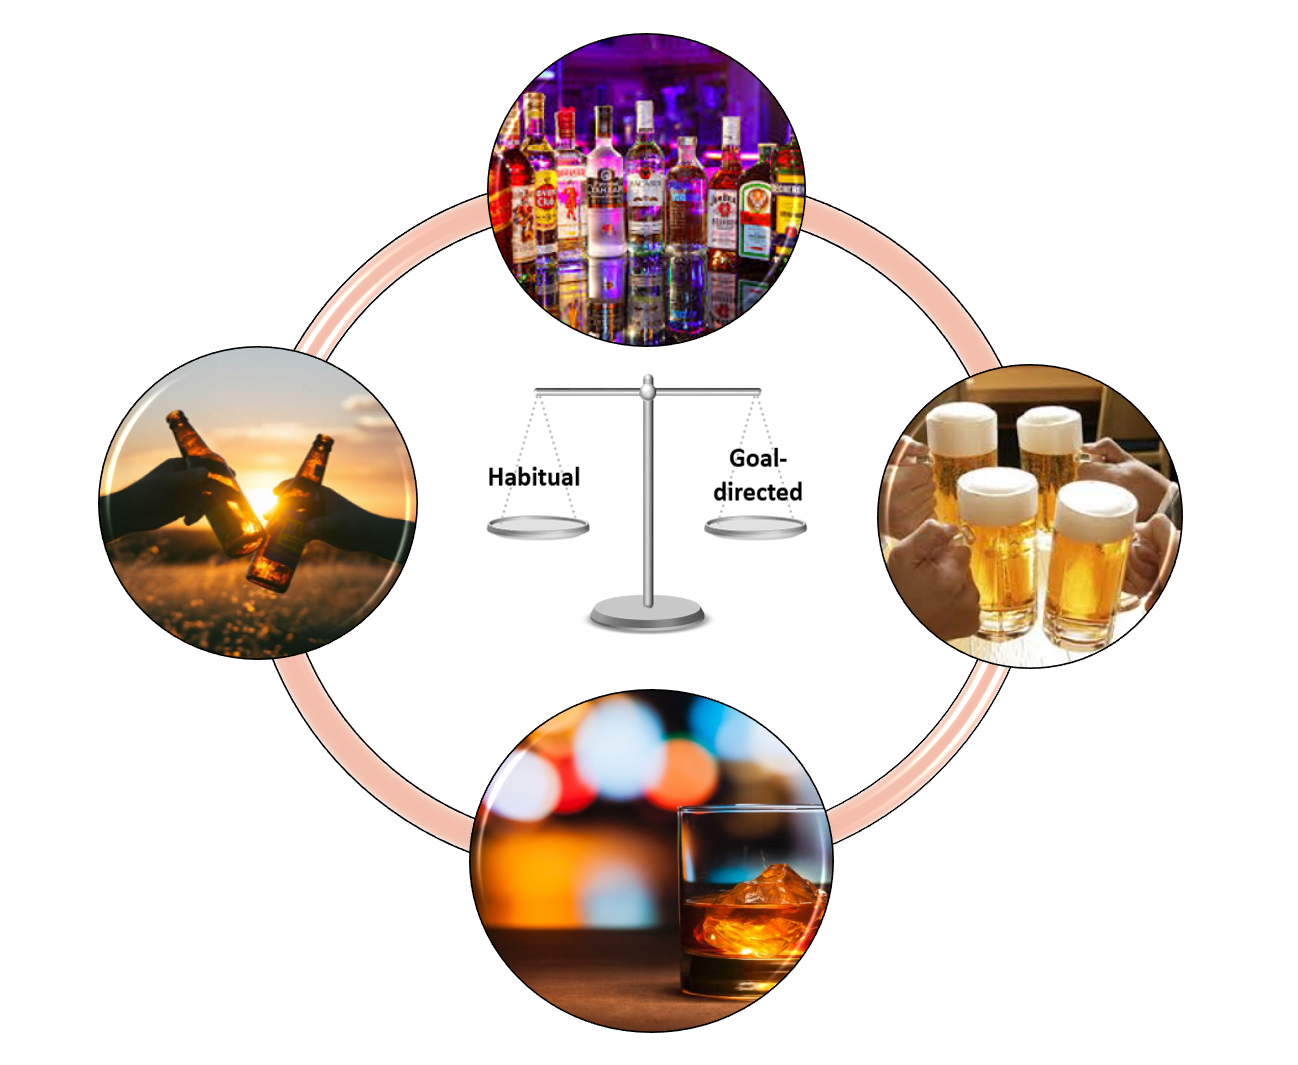
\includegraphics[scale=0.35]{images/Zyklus.PNG}
        %\caption{\small{Dual control approach.}}
    \end{figure}
\end{frame}

%%%%%
\begin{frame}{Dual control approach in alcohol dependence}
    \begin{figure}
       
        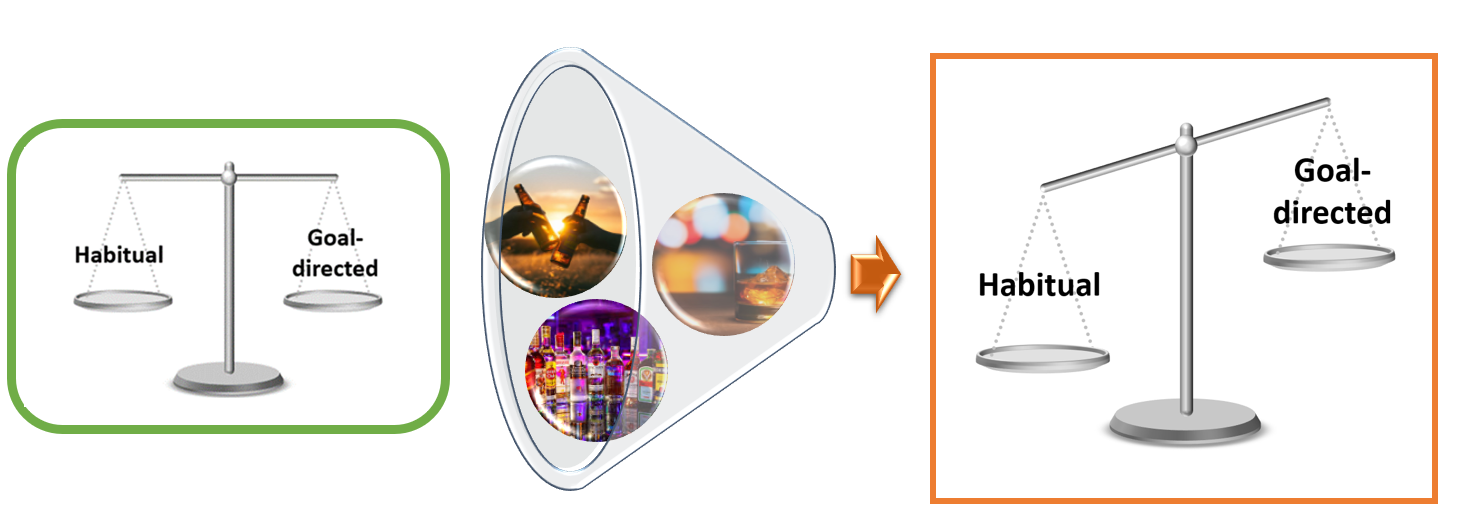
\includegraphics[scale=0.41]{images/bZyklus.PNG}
         \caption{Imbalance in the dual control approach.}
    \end{figure}
\end{frame}

%--------------------------------------
%%%%%

\begin{frame}{Alcohol approach avoidance Task (aAAT)}
Probanden wurden implizit trainiert, Vermeidungsbewegung (durch Wegdrücken eines Joysticks) als Reaktion auf alkoholische Bilder durchzuführen.
 				\begin{figure}
   				  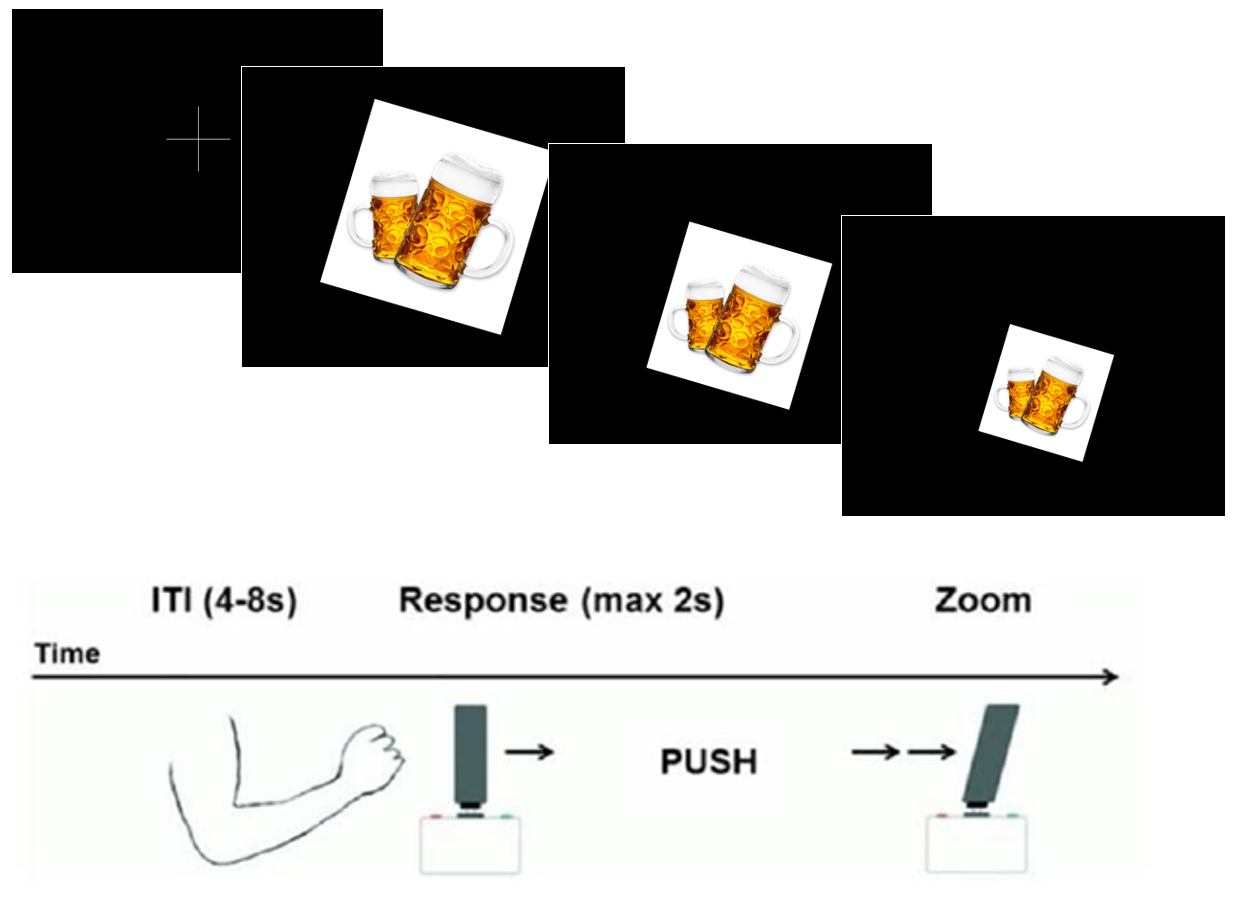
\includegraphics[scale=0.3]{images/AAT_new.PNG}
   				\caption{\small{Scheme of the cognitive-bias modification training.}}
	\end{figure}
\end{frame}

%%%%%%
\subsection{DAS PROJEKT LEAD}
\begin{frame}{Research project}
\begin{columns}
\begin{column}{6cm}
\begin{itemize}
\item Lernen und Habituierung als Prädiktoren für die Entwicklung und Aufrechterhaltung des Alkoholismus
\vspace{2mm}
\item Bizentrische DFG-geförderte fMRT-Studie in Zusammenarbeit mit der Technischen Universität Dresden und dem Universitätsklinikum Carl Gustav Carus, Dresden
\end{itemize}
\end{column}
\begin{column}{5cm}
\begin{figure}
    
\includegraphics[scale=0.7]{images/Clogo.PNG}\\
    \vspace{2mm}
   
\includegraphics[scale=0.7]{images/dres.jpg}
\end{figure}
\end{column}
\end{columns}
\end{frame}

%%%%%%%


\subsection{MASTER THESIS}
%%
	\begin{frame}{Working memory and alcohol dependence}

	\begin{itemize}
	\item Exekutive Verhaltenskontrolle, Selbstregulierung, Informationsverarbeitung
  	\item \textbf{Beeinträchtigungen} des Arbeitsgedächtnisses in Alkoholabhängigen beobachtet
  	  	\item \textbf {Chronischer Alkoholkonsum interferiert} des Weiteren mit...
  	  	\begin{itemize}
  	\item \textbf {präfrontale kortikale Funktionsfähigkeit
  	    \item zielgerichtetes Verhalten }
  	   \\(Rottschy et al., 2012\cite{Rottschy.2012}; Wiers et al. 2017\cite{Wiers.2017})
  	\end{itemize} 
  	 \item Bildgebende Studien: Informationsverarbeitung erfordert eine \textbf{kompensierende erhöhte neuronale Aktivierung} (Charlet et al.,2014\cite{Charlet.2014}).
 		\end{itemize}
 		\cite{Crews.2005} \cite{Dougherty.2016} \cite{Eberl.2013}
	\end{frame}
%%%%%
%-------------------------------------------------------------	
%%%%%%%%%%%%%%%%%%%%%%%%%%%%%%%%%%%%%%%%%%%%%%%%%%%%%%%%%%%%%%%

\section{Method}
\subsection{MASTER THESIS}
\begin{frame}{N-back task}
	\begin{figure}
   			 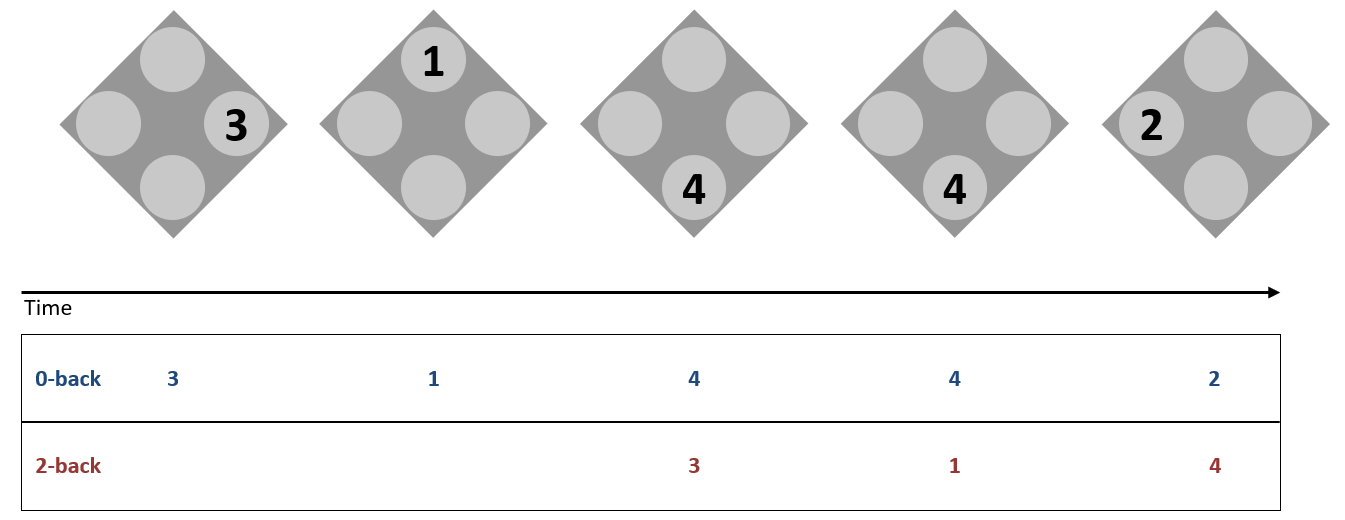
\includegraphics[scale=0.43]{images/n-back_logik.PNG} \\
   			 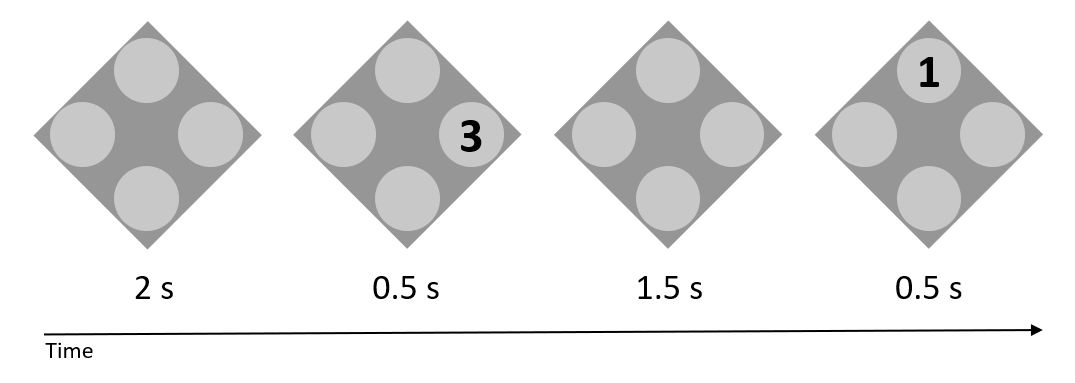
\includegraphics[scale=0.3]{images/n-back_timeline.PNG}
   					\caption{\tiny{ Scheme of the fMRI n-back working memory paradigm (Callicott et al. 1999\cite{Callicott.1999}).Two conditions (0-back and 2-back) were assessed
in four alternating blocks, each lasting 30 seconds.}}
\end{figure}
\end{frame}
%%%%%

\begin{frame}{Huh?}
\hspace{7mm}
 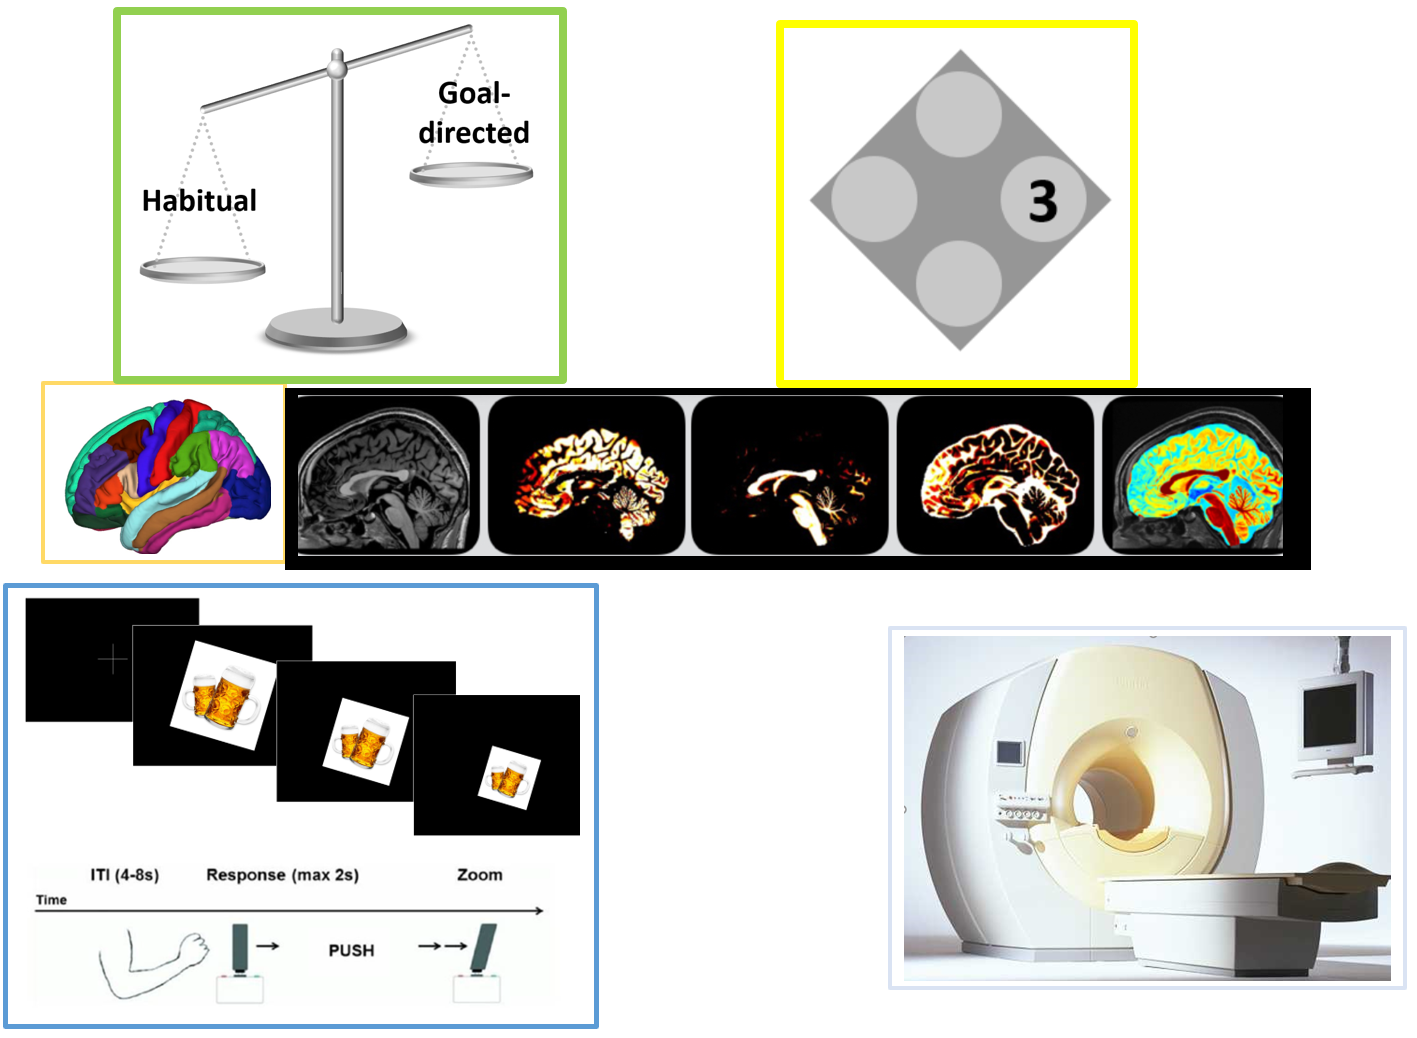
\includegraphics[scale=0.37]{images/huh2.PNG}
\end{frame}
%%%%%
\begin{frame}{Experimental design}
\begin{figure}
       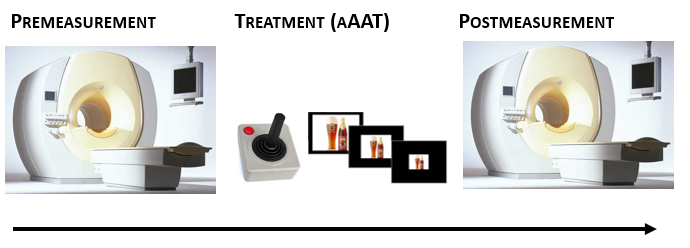
\includegraphics[scale=0.55]{images/expdesign.PNG}
       \caption{Experimental design in the course of time.}
 
\end{figure}
\end{frame}

%%%%
\begin{frame}{Research idea}
\begin{block}{\textbf{ Zielsetzung}}
 Untersuchung von Unterschieden zwischen alkoholabhängigen Patienten und gesunden Kontrollen während der n-back Aufgabe hinsichtlich 
\begin{itemize}
    \item der Arbeitsgedächtnisleistung 
    \item  neuronaler Aktivierungsmuster 
    %\item No existing publications whether these differences change by aAAT over time
  	%\item Evidence that working memory capacity moderates training efficacy with the aAAT (Sharbanee et al. 2014)
    \end{itemize}
    \end{block}
\begin{exampleblock}{\textbf{{Datenformate}}}
 Analyse von Verhaltens- und Imagingdaten (fMRT)
\end{exampleblock}
\end{frame}

%%%
\begin{frame}{Research idea}
\begin{block}{\textbf{Hypothesen}}
\hspace{7mm}
 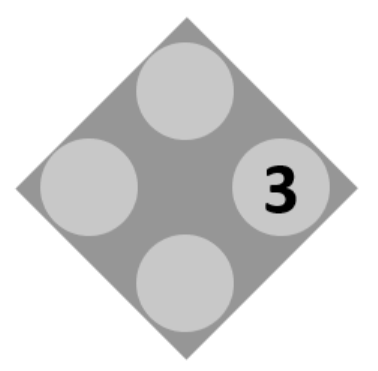
\includegraphics[scale=0.28]{images/nback.PNG}
 \hspace{4mm}
 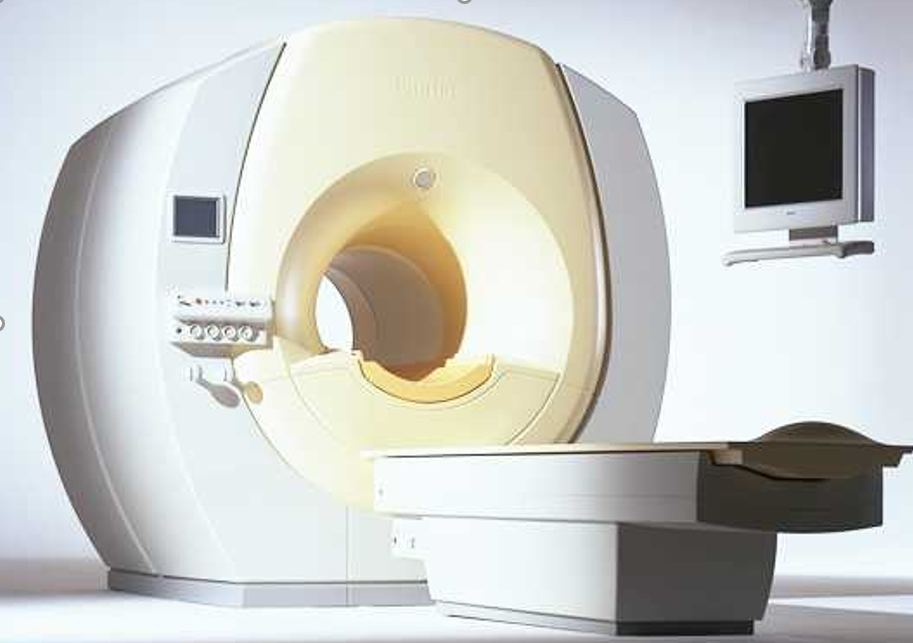
\includegraphics[scale=0.15]{images/scanner.PNG}
 \hspace{4mm}
 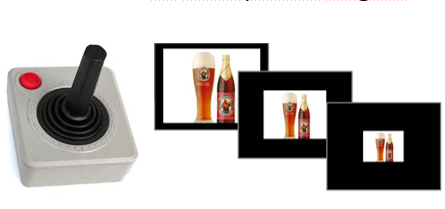
\includegraphics[scale=0.48]{images/aat.PNG}
{\begin{itemize}
\item \small N-back Performance: AD = HC \footnote{\footnotesize{(AD = alcohol dependents, HC = healthy controls)\cite{Charlet.2014}}}
\item \small Neuronale Aktivierung: AD > HC
\item \small Intervention AAT 2-back Performance: verum > placebo
\item \small Intervention AAT neuronale Aktivierung: verum < placebo
\item \small Prä-Post-Vergleich 2-back Performance: T2 > T1
\item \small Prä-Post-Vergleich neuronale Aktivierung: T2 < T1
\end{itemize}}
\end{block}
\end{frame}


%%%%%
\begin{frame}{Sample}
\begin{figure}
    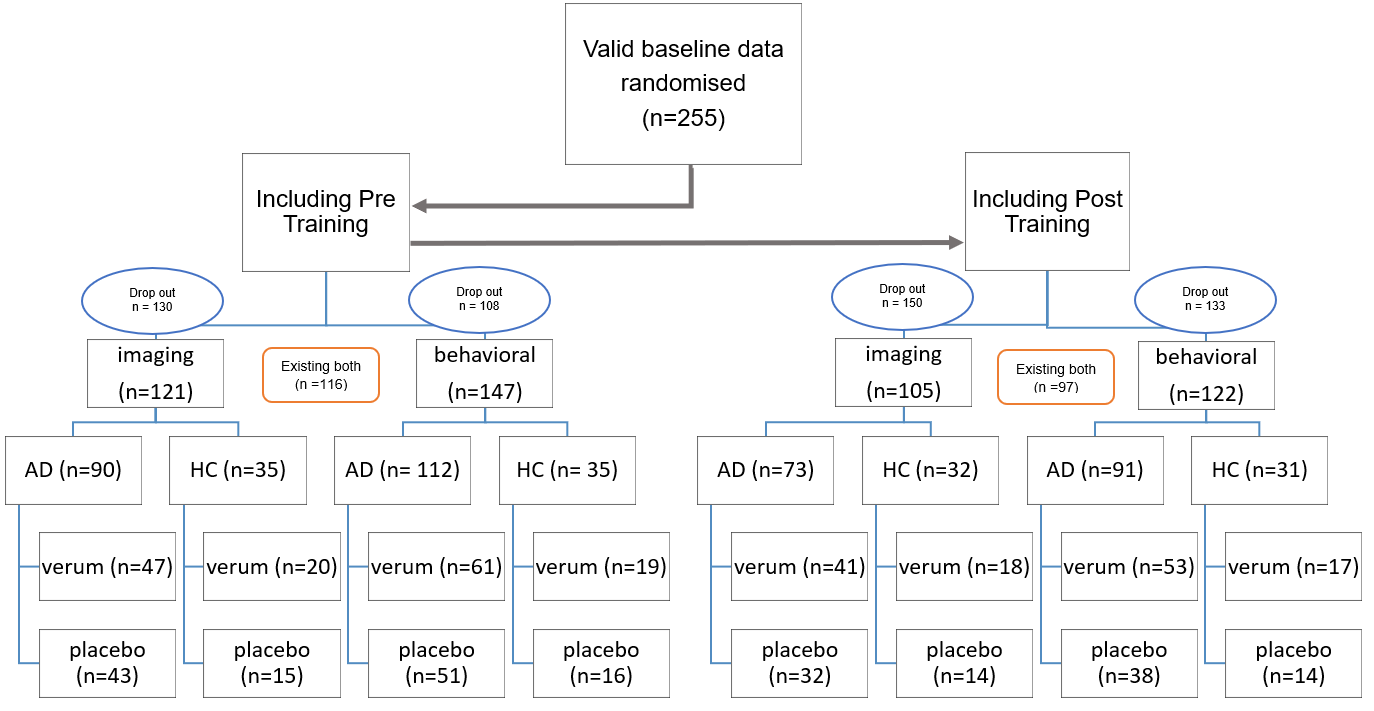
\includegraphics[scale=0.44]{images/Sample.PNG}
    \caption{\tiny{Description of sample sizes and drop outs at each stage of the analysis procedure. AD = Alcohol dependents, HC = Healthy controls, VE = Verum, PLA = Placebo, behavioral = n-back data.}}
\end{figure}
\end{frame}
%%%%%


\begin{frame}{Inclusion criteria}
\begin{itemize}
    \item (1)	Men and women aged 18-65 years
\item (2)	AUD according to ICD-10 and alcohol-use disorder according to DSM-5
\item (3)	Minimum of 72 hours of abstinence, maximum of 21 days of abstinence
\item (4)	Minimum of three years with AUD
\item (5)	Low severity of withdrawal symptoms (CIWA =0 for three consecutive days)
\item (6)	Ability to provide fully informed consent and to use self-rating scales
\item (7)	Sufficient understanding of the German language
\end{itemize}
\end{frame}
%%%%

\begin{frame}{Exclusion criteria}
\small
\begin{itemize}
    \item (1)	Lifetime history of DSM-IV diagnosis
\item (2)	Current threshold DSM-IV diagnosis [(hypo)manic episode, major depressive disorder, generalized anxiety disorder, PTSD, borderline personality disorder]
\item (3)	Substance dependence other than alcohol or nicotine dependence
\item (4)	Current substance use other than nicotine and alcohol 
\item (5)	History of severe head trauma or other severe central neurological disorder 
\item (6)	Pregnancy or nursing infants
\item (7)	Any alcohol intake within the last 24 hours
\item (8)	Use of medications or drugs known to interact with the CNS within the last 10 days
\end{itemize}   
\end{frame}

%%%%

\begin{frame}{Sample}
\begin{exampleblock}{Descriptive data}
\begin{itemize}
\item Age: 18 - 65
\item Right-handed
\item Education
\item Lifetime alcohol consumption in kilograms
\item AUDIT
\item Smoker status
\item BDI
\item STAI
\end{itemize}
\end{exampleblock}
\end{frame}
%%%%%

\begin{frame}{Behavioral data}
\begin{block}{Test differences in performance (hit miss incorrect and  RT)}
\small
\begin{itemize}
\item \textbf{ANCOVAs} with hit, miss, incorrect rates in the 2 back condition as dependent variable and factor %group (AD, HC) as independent variable
\item \textbf{Kruskal-Wallis H test} for the not-normally distributed hit/ miss/ incorrect rates in the 0-back %condition 
\item \textbf{Repeated measurement ANCOVA} with the mean response time of hits with
\item \textbf{Performance decrement} within each subject\\ high \textit{negative} values indicate worsening from %the 0-back to the 2-back condition 
\item Additionally \textbf{General Linear Mixed Effects Models (GLMER)} \\
between-subject factor group (AD, HC) \\
within-subject factor condition (0-back, 2-back)
    \end{itemize}
    \end{block}
\end{frame}

%\begin{frame}{Imaging data}
%\begin{itemize}
%    \item Imaging data will be analysed with SPM12
%    \item After pre-processing and artefact reduction the EPI images will be analysed in an block related manner using the general linear model approach (GLM) approach at the first (single subject) and second (group) level
%\end{itemize}
%\end{frame}



\section{Results}
\subsection{BEHAVIOURAL DATA}
%\begin{frame}{Behavioral data: Performance decrement hit rates}
%\begin{figure}
%    \includegraphics[width=0.53\textwidth, top]{T1_Decrement.png}
%    \includegraphics[width=0.53\textwidth, top]{T2_Decrement_.png}
%    \caption{\tiny{Performance decrement at both time points (t1, t2).}}
%\end{figure}
%\end{frame}

\begin{frame}{Hit rates in percent}
\begin{figure}
\centering
     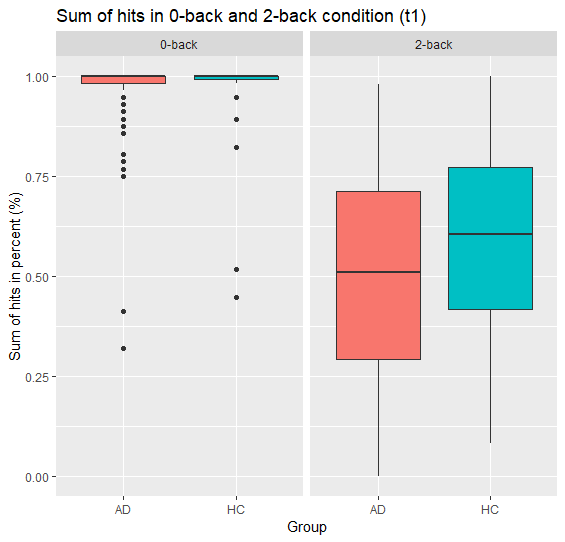
\includegraphics[scale=0.43]{images/T1_Hit.png}
    %\includegraphics[width=0.53\textwidth, top]{T2_Hit.png}
    \caption{\tiny{Hit rates at the premeasurement (t1). }}
    \end{figure}
\end{frame}
%%%%

\begin{frame}{Reaction time}
\begin{figure}
     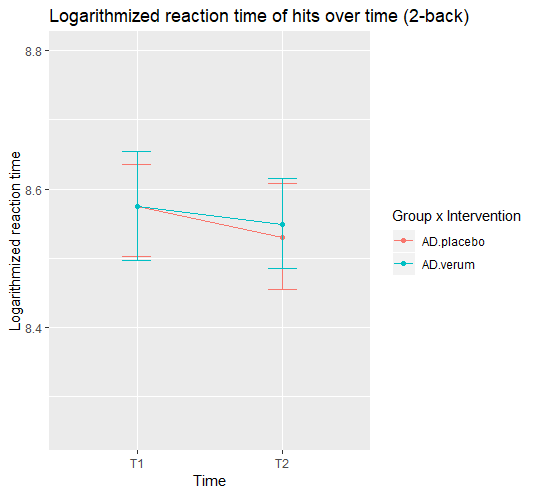
\includegraphics[scale=0.42]{images/T1T2_Interaction_AD.png} 
     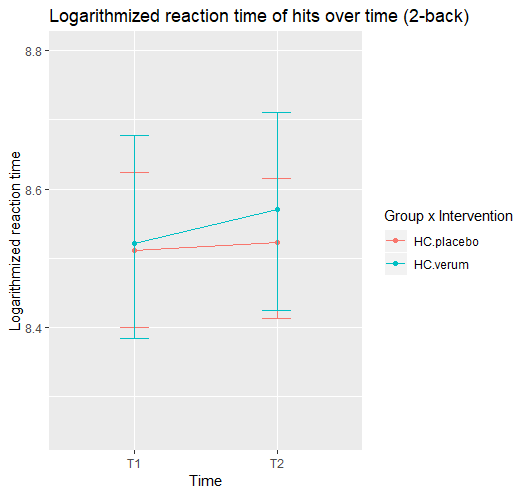
\includegraphics[scale=0.42]{images/T1T2_Interaction_HC.png} 
    \caption{\tiny{T1- T2 comparisons.}}
    \end{figure}
\end{frame}

%%%%%
\begin{frame}{Summary of group comparisons}
\begin{figure}
     \includegraphics[scale=0.40]{images/Table_BehavRes.PNG}
\end{figure}
\end{frame}



%\begin{frame}{Behavioral data: Reaction times}
%\begin{figure}
%\hspace*{-0.5cm}
   % \includegraphics[width=0.53\textwidth, top]{T1_RT_Hit.png}
  %  \includegraphics[width=0.53\textwidth, top]{T2_RT_Hit.png}
 %   \caption{\tiny{Reaction times at both time points (t1, t2). }}
%\end{figure}
%\end{frame}

%\begin{frame}{Behavioral data}
%\begin{figure}
%\hspace*{-0.5cm}
%    \includegraphics[width= 1\linewidth, height = 5.5 cm, top]{Table_BehavRes.PNG}
%    \caption{\tiny{Performance measures during the 0-back and 2-back condition of the fMRI n-back task. (a) Accuracy rates in percent. (b) Response times in milliseconds.}}
%\end{figure}
%\end{frame}

%\begin{frame}[fragile]{Imaging data}
%\end{frame}

%%%%
\subsection{IMAGING DATEN}
\begin{frame}{FMRI data analysis}
\begin{columns}
\begin{column}{6cm}
\begin{itemize}
\small
    \item Preprocessing and analyses with SPM12
    \item Two-level procedure: First and Second Level Analysis: \\
    Block design in context of the GLM 
    \item Linear contrast images computed for 2-back-0-back for each subject
    \item Literature-based analysis on key brain structures (ROI, family wise-error corrected) 
\end{itemize}
\end{column}
\begin{column}{5cm}
  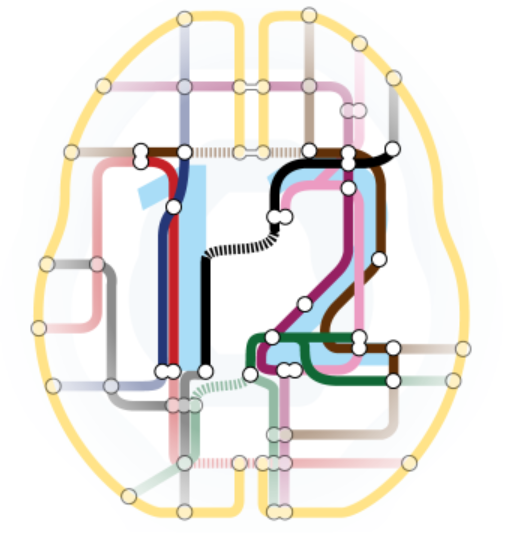
\includegraphics[scale=0.40]{images/SPM.PNG}
\end{column}
\end{columns}
\end{frame}

%%%%
\begin{frame}{2nd Level Results}
\centering
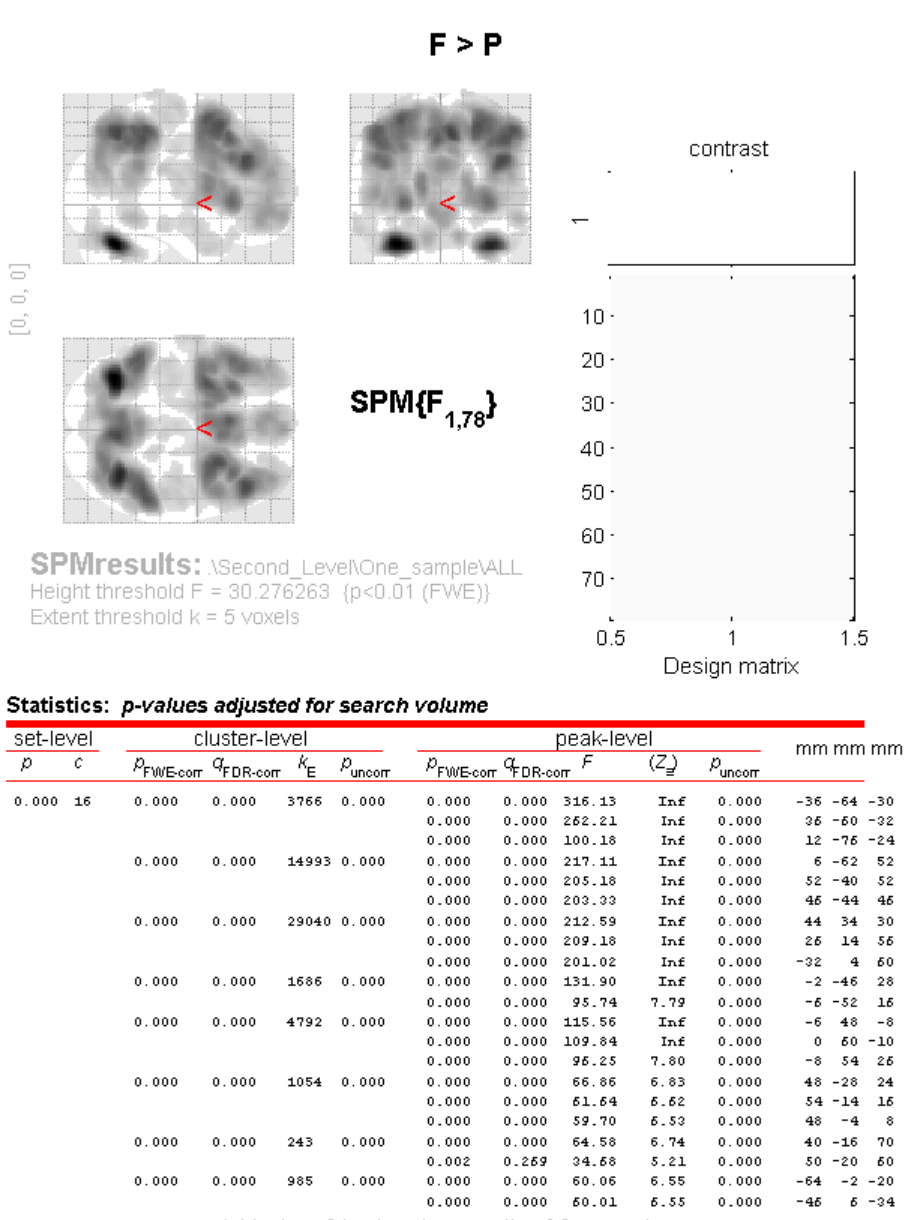
\includegraphics[scale=0.3]{images/SPM2.PNG}
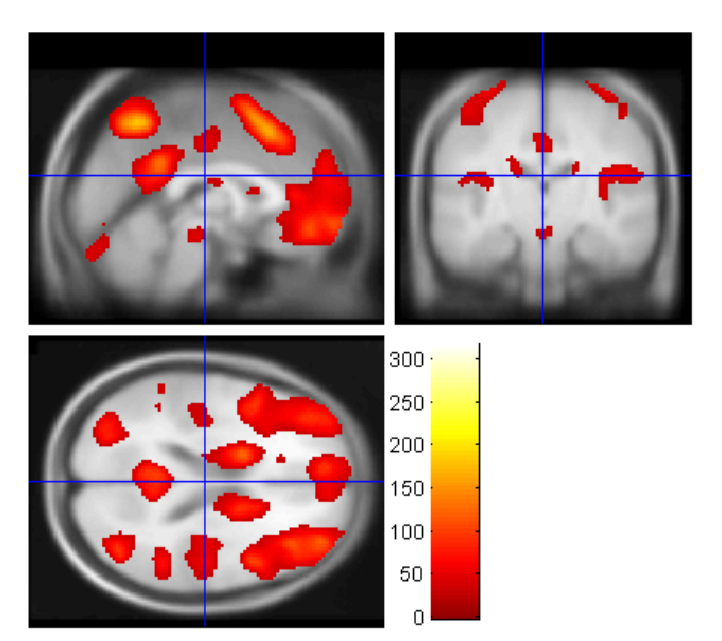
\includegraphics[scale=0.3]{images/SPM1.PNG} 
\end{frame}

%%%%
\begin{frame}{2nd Level Results}
\begin{figure}
\centering
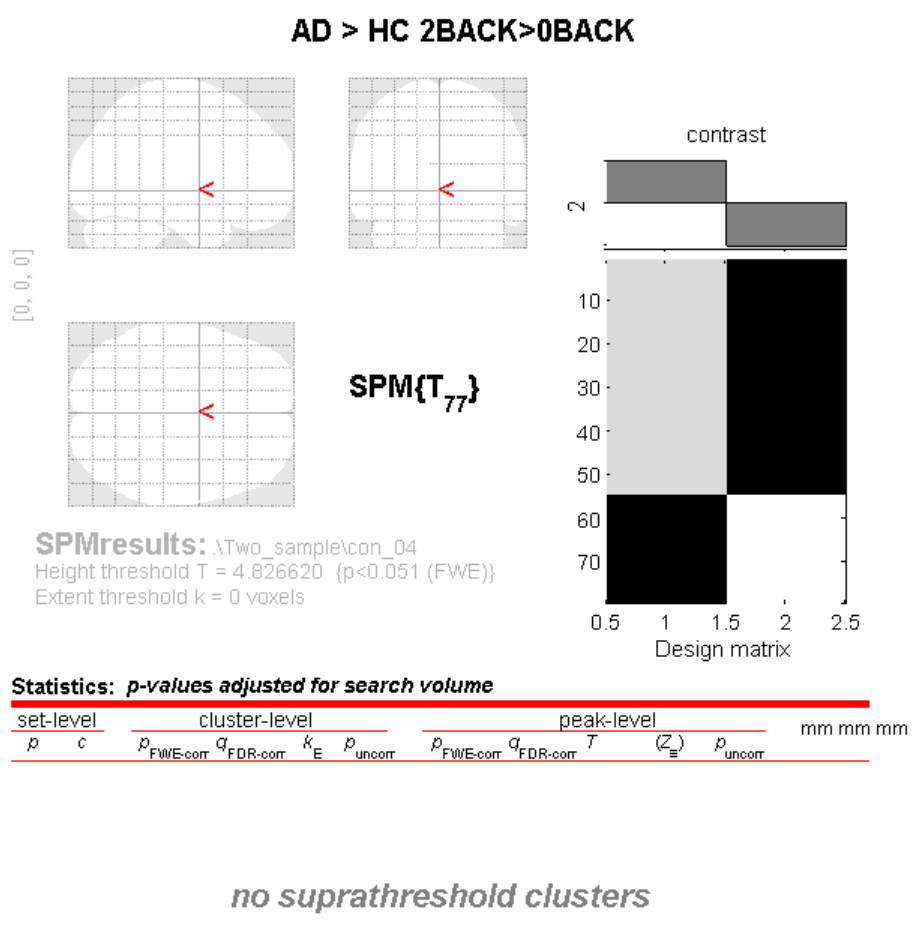
\includegraphics[scale=0.37]{images/SPM3.PNG}
\caption{\tiny{T1 - two sample t-test [AD - HC]}}
\end{figure}
\end{frame}


%%%%%
\begin{frame}{Design matrix}
\centering
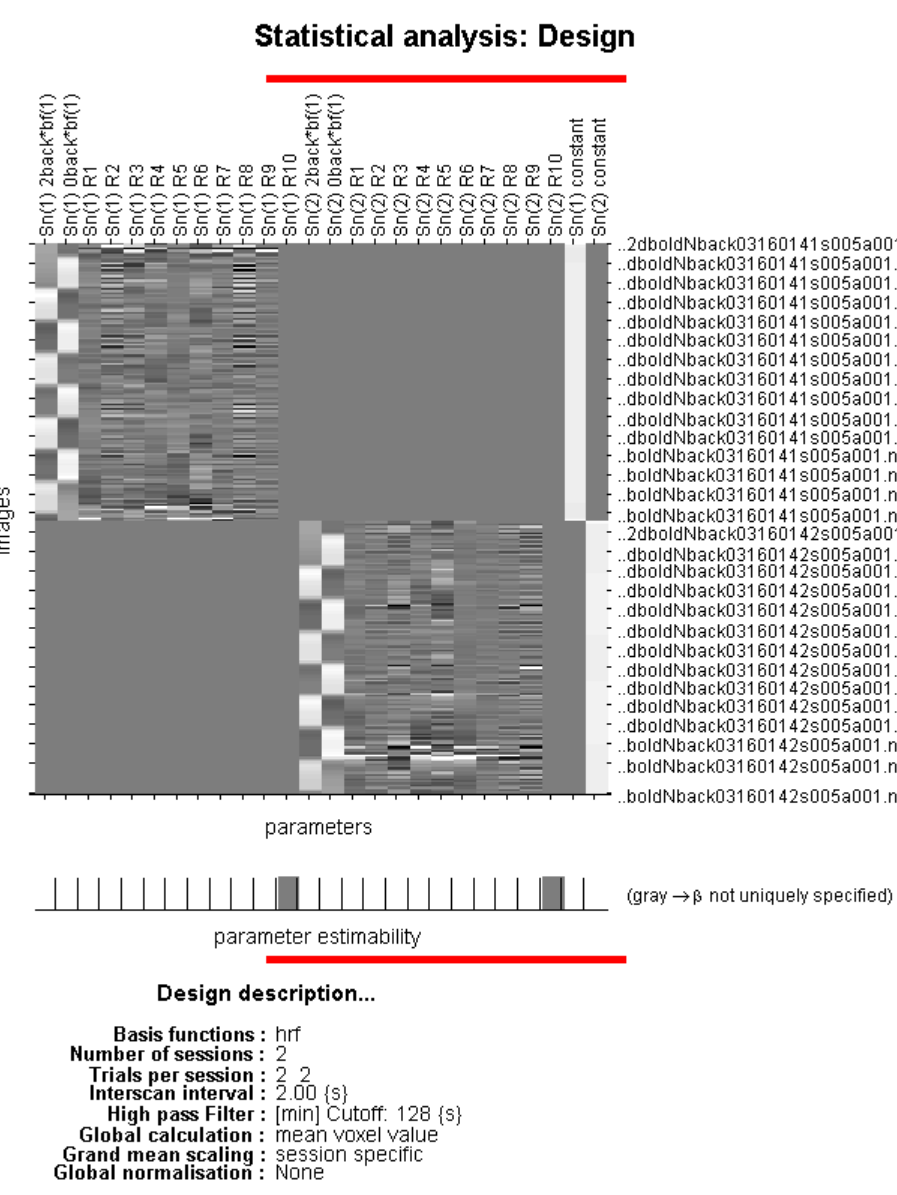
\includegraphics[scale=0.40]{images/DesiMatr.PNG}
\end{frame}

%%%%
\begin{frame}{Conclusion for now}
\begin{block} {}
    \begin{itemize}
            \item Beide Gruppen (AD - HC, verum - placebo) zeigen keine signifikanten Unterschiede in der Performance n-back Aufgabe.
        \item Keine signifikanten Unterschiede in der neuronalen Aktivierung im Gruppenvergleich (AD - HC, verum - placebo)
            \end{itemize}
        \end{block}
        \end{frame}
 %%%%      
\begin{frame}
    \centering
    \Huge{\textcolor{darkblue}{Thank you for your attention!}}
    %\begin{figure}[ht]
    %\includemovie[
    %poster,
    %text={\small(Loading mathgif.mp4)}
%]{6cm}{6cm}{mathgif.mp4}
%\end{figure}
\end{frame}        

%____________________________________________
\section{References}
%%%%
\begin{frame}{Relevant literature}
\insert{bibliography}
\tiny \bibliography{Bibliography.bib}
\bibliographystyle{nar}

\end{frame}
\end{document}